%
% icos.tex -- I(t) cos\omega t auf dem Einheitskreis
%
% (c) 2018 Prof Dr Andreas Müller, Hochschule Rapperswil
%
\documentclass[tikz,12pt]{standalone}
\usepackage{times}
\usepackage{amsmath}
\usepackage{txfonts}
\usepackage[utf8]{inputenc}
\usepackage{graphics}
\usepackage{color}
\usepackage{pifont}
\usetikzlibrary{arrows,intersections,math,calc}
\begin{document}

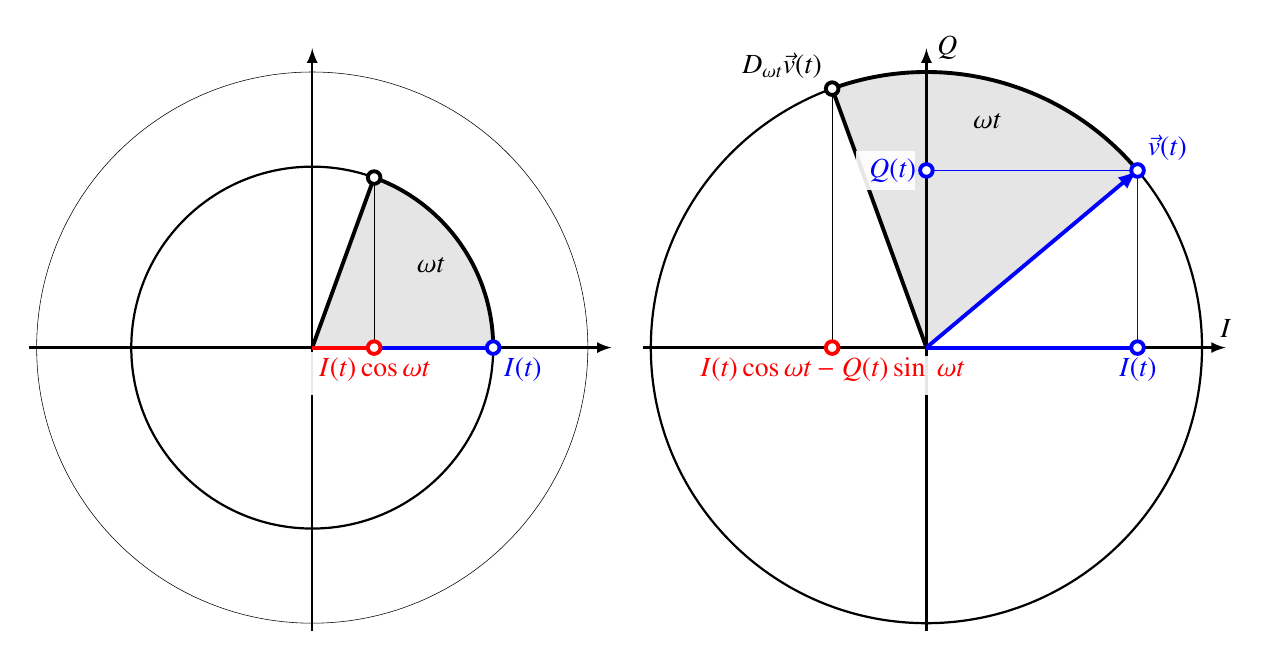
\begin{tikzpicture}[>=latex,thick]

\def\r{3.5}
\def\a{70}
\def\b{40}
\pgfmathparse{3*cos(\b)}
\xdef\I{\pgfmathresult}

\draw[line width=0.2pt] (0,0) circle[radius=\r];

\fill[color=black!10] (0,0) -- (\I,0) arc (0:\a:\I) -- cycle;
\node at ({\a/2}:{0.8*\I}) {$\omega t$};

\draw[line width=0.2pt] (\a:\I) -- ({\I*cos(\a)},0);

\draw[color=black,line width=1.4pt] (0,0)--(\a:\I);

\draw (0,0) circle[radius=\I];

\draw[color=black,line width=1.4pt] (0:\I) arc (0:\a:\I);

\fill[color=white]                  (\a:\I) circle[radius=0.08];
\draw[color=black,line width=1.4pt] (\a:\I) circle[radius=0.08];

\draw[->] ({-\r-0.1},0) -- ({\r+0.3},0); % coordinate[label={$I$}];
\draw[->] (0,{-\r-0.1}) -- (0,{\r+0.3}); % coordinate[label={right:$Q$}];

\draw[color=blue,line width=1.4pt] (0,0) -- (\I,0);
\fill[color=white]                 (\I,0) circle[radius=0.08];
\draw[color=blue,line width=1.4pt] (\I,0) circle[radius=0.08];
\node[color=blue] at (\I,0) [below right] {$I(t)$};

\draw[color=red,line width=1.5pt] (0,0) -- ({\I*cos(\a)},0);
\fill[color=white]                ({\I*cos(\a)},0) circle[radius=0.08];
\draw[color=red,line width=1.4pt] ({\I*cos(\a)},0) circle[radius=0.08];
\fill[color=white,opacity=0.9] (-0.2,-0.6) rectangle (0.2,-0.05);
\node[color=red] at ({\I*cos(\a)},0) [below] {$I(t)\cos \omega t$};

\begin{scope}[xshift=7.8cm]

\fill[color=black!10] (0,0) -- (\b:\r) arc (\b:{\a+\b}:\r) -- cycle;

\draw (0,0) circle[radius=\r];
\draw[line width=1.4pt] (\b:\r) arc (\b:{\a+\b}:\r);

\node at ({\b+\a/2}:{0.85*\r}) {$\omega t$};

\draw[color=black,line width=0.2pt] ({\a+\b}:\r) -- ({\r*cos(\a+\b)},0);

\draw[->] ({-\r-0.1},0) -- ({\r+0.3},0) coordinate[label={$I$}];
\draw[->] (0,{-\r-0.1}) -- (0,{\r+0.3}) coordinate[label={right:$Q$}];

\draw[color=blue,line width=0.2pt] (\b:\r)--({\r*cos(\b)},0);
\draw[color=blue,line width=0.2pt] (\b:\r)--(0,{\r*sin(\b)});

\draw[color=blue,line width=1.4pt] (0,0)--({\r*cos(\b)},0);
\fill[color=white]                 ({\r*cos(\b)},0) circle[radius=0.08];
\draw[color=blue,line width=1.4pt] ({\r*cos(\b)},0) circle[radius=0.08];
\node[color=blue] at ({\r*cos(\b)},0) [below] {$I(t)$};

\fill[color=white] ({\r*cos(\a+\b)},0) circle[radius=0.08];
\draw[color=red,line width=1.4pt] ({\r*cos(\a+\b)},0) circle[radius=0.08];

\draw[color=black,line width=1.4pt] (0,0) -- ({\a+\b}:\r);
\fill[color=white]                ({\a+\b}:\r) circle[radius=0.08];
\draw[color=black,line width=1.4pt] ({\a+\b}:\r) circle[radius=0.08];

\draw[->,color=blue,line width=1.4pt] (0,0) -- (\b:\r);
\fill[color=white] (\b:\r) circle[radius=0.08];
\draw[color=blue,line width=1.4pt] (\b:\r) circle[radius=0.08];

\fill[color=white]                 (0,{\r*sin(\b)}) circle[radius=0.08];
\draw[color=blue,line width=1.4pt] (0,{\r*sin(\b)}) circle[radius=0.08];

\fill[color=white,opacity=0.9]
	(-0.9,{\r*sin(\b)-0.25}) rectangle (-0.15,{\r*sin(\b)+0.25});
\node[color=blue] at (0,{\r*sin(\b)}) [left] {$Q(t)$};

\node at ({\a+\b}:\r) [above left] {$D_{\omega t}\vec{v}(t)$};

\fill[color=white,opacity=0.9]
	({\r*cos(\a+\b)-2},-0.6) rectangle ({\r*cos(\a+\b)+2},-0.11);
\node[color=red] at ({\r*cos(\a+\b)},0) [below]
	{$I(t)\cos \omega t-Q(t)\sin \omega t$};

\node[color=blue] at (\b:\r) [above right]
	{$\vec{v}(t)$};

\end{scope}

\end{tikzpicture}

\end{document}

